\pdfminorversion=5
\pdfobjcompresslevel=2

\RequirePackage[l2tabu, orthodox]{nag}

\documentclass[sigplan]{acmart}

\usepackage[T1]{fontenc}
\usepackage[utf8]{inputenc}

\usepackage{microtype}
\usepackage{listings}
\usepackage{color}
\usepackage{xspace}
\usepackage{balance}
\usepackage{todonotes}
\usepackage[all]{nowidow}
\usepackage{tikz}
\usepackage[scaled]{beramono}
\usepackage{booktabs}
%\usepackage[bookmarks=false,colorlinks=true,allcolors=black,breaklinks]{hyperref}
\usepackage{cleveref} % Keep me last so that I can
                      % reset other counters

% Copyright
%\setcopyright{none}
%\setcopyright{acmcopyright}
%\setcopyright{acmlicensed}
%\setcopyright{rightsretained}
%\setcopyright{usgov}
%\setcopyright{usgovmixed}
%\setcopyright{cagov}
%\setcopyright{cagovmixed}


% DOI
%\acmDOI{10.475/123_4}

% ISBN
%\acmISBN{123-4567-24-567/08/06}

%Conference
\acmConference[SLE'18]{International Conference on Software Language Engineering}{November 2018}{Boston, MA, USA}
\acmYear{2018}
\copyrightyear{2018}

\acmPrice{15.00}

%\acmBadgeL[http://ctuning.org/ae/ppopp2016.html]{ae-logo}
%\acmBadgeR[http://ctuning.org/ae/ppopp2016.html]{ae-logo}

\hypersetup{%
	pdftitle={},
	pdfauthor={},
	pdfkeywords={}
}

% Usual suspects
\newcommand*{\ie}{i.e.,\@\xspace}
\newcommand*{\eg}{e.g.,\@\xspace}
\newcommand*{\cf}{cf.\@\xspace}

\makeatletter
\newcommand*{\etc}{%
	\@ifnextchar{.}%
	{etc}%
	{etc.\@\xspace}%
}
\makeatother

\newcommand*{\de}{$\Delta$\@\xspace}
\newcommand*{\ds}{$\Delta$s\@\xspace}
\newcommand*{\db}{$\Delta$-based\@\xspace}
\newcommand*{\M}{\mathcal{M}}

\newcommand*{\diff}{\textit{diff}\@\xspace}
\newcommand*{\patch}{patch\@\xspace}
\newcommand*{\prism}{\textsc{Prism}\@\xspace}

% Listings
\definecolor{keywordscolor}{RGB}{127, 0, 85}
\definecolor{stringcolors}{RGB}{42, 0, 255}
\definecolor{commentscolor}{RGB}{63, 127, 95}
\definecolor{annotationscolor}{RGB}{100, 100, 100}
\definecolor{lstbgcolor}{RGB}{245, 245, 245}

% Custom Java
\lstset{
	language=Java,
	%	mathescape=true,
	literate={->}{$\rightarrow$}{1},
	keywordstyle=\color{keywordscolor}\bfseries,
	commentstyle=\color{commentscolor},
	stringstyle=\color{stringcolors},
	basicstyle=\ttfamily\tiny,
	captionpos=b,
	numbers=left,
	%	backgroundcolor=\color{lstbgcolor},
	%	framexleftmargin=20pt,
	xleftmargin=17pt,
	aboveskip=\bigskipamount,
	belowskip=\bigskipamount,
	%	frame=tb,
	tabsize=2,
	breaklines=true
}

% Rascal
\lstdefinelanguage[]{Rascal}[]{Java}
{
	morecomment=[l]{\@},
	morekeywords={alias, tuple, lrel, data, str, value, int, list}
}

\usetikzlibrary{shapes.callouts, shadows}
\tikzset{author comment/.style={draw, fill=white, thick, drop shadow}}

\newcommand{\Comment}[3]{%
	\ifthenelse{\boolean{CommentON}}{%
		\raisebox{-.5ex}
		{\tikz
			\node[x=1ex, y=1ex, inner sep=.5ex,
			rectangle callout,
			callout pointer width=.7ex,
			callout relative pointer={(1.5,-0)},
			author comment]
			{\footnotesize\textsf{#1}};}~%
		\textsf{[}\,\textcolor{#2}{#3}\,\textsf{]}\xspace
	}{} %else
}

\newcommand{\td}[1]{\Comment{TD}{blue}{#1}}
\newcommand{\fc}[1]{\Comment{FC}{red}{#1}}


\newboolean{CommentON}
\setboolean{CommentON}{true} % to disable the comments set CommentON to false in the main doc

\begin{document}
\title{``\emph{Free the languages!}''}
%\titlenote{Models are synchonized, not DSLs, though}
\subtitle{Language Engineering across Technological Boundaries}
%\subtitlenote{The full version of the author's guide is available as
%		\texttt{acmart.pdf} document}

\author{ALE}
%\authornote{Dr.~Trovato insisted his name be first.}
%\orcid{1234-5678-9012}
\affiliation{%
	\institution{ALE}
%	\streetaddress{P.O. Box 1212}
%	\city{Dublin}
%	\state{Ohio}
%	\postcode{43017-6221}
}
\email{ale@ale.org}

% The default list of authors is too long for headers.
%\renewcommand{\shortauthors}{B. Trovato et al.}

\begin{abstract}
Domain-Specific Languages (DSLs) manifest themselves in remarkably diverse shapes, ranging from internal DSLs embedded as a mere fluent API within a programming language, to external DSLs with dedicated syntax and tool support.
% engineered using one of many language workbenches.
%
Although different shapes have different pros and cons, combining them for a single language is problematic:~language designers usually commit to a particular shape early in the design process and it is hard to reconsider this choice later on.
%
%Theoretically, this diversity should enable language designers to combine the strengths of multiple language engineering technologies in the development of a single DSL and enable language users to manipulate their abstractions in the most appropriate shape for the task at hand (\eg~domain modeling vs. system integration).
%In practice, however, combining multiple language implementation techniques is problematic.
%Language designers usually commit to a particular technology (\eg~Spoofax, EMF, Racket) and a particular shape (\eg~internal, external, API) early in the design process and this choice can hardly be reconsidered later on.
%
In this \emph{new ideas} paper, we envision a language engineering approach enabling (i) language users to manipulate their abstractions in the most appropriate shape according to the task at hand, and (ii) language designers to combine the strengths of different technologies for a single DSL. 
%support of multiple shapes for a single DSL to better fit the various tasks to be performed with it. \td{Meh}
%report on early experiments and lessons learned building an incremental synchronization mechanism for \emph{metamorphic DSLs}.
%
We report on early experiments and lessons learned building \prism, an incremental technique for synchronizing multiple shapes of a DSL.
We illustrate its applicability in the engineering of a simple shape-diverse DSL implemented in Rascal, EMF, and Java.
%Metamorphic DSLs are languages whose different constituents (syntax, semantics, tools) can be implemented using various language engineering technologies and which can adapt their shape to a particular user or task.
%Taking as an example a simple metamorphic FSM language implemented simultaneously in three technological spaces (Rascal, EMF, a fluent API in Java), we show how the same FSM models can be manipulated indifferently under various shapes (a textual program in Rascal, a graphical projection in EMF, a Java AST).
%This opens up the possibility to, \eg animate an FSM model in EMF while it is executed by an interpreter written in Rascal.
%
We hope that our initial contribution will raise the awareness of the community regarding these notions, and that the challenges we identify encourage future research.
%We intend to raise the awareness of the community on these notions, identify some of the challenges we encountered along the way, and encourage future investigations.
\end{abstract}


%
% The code below should be generated by the tool at
% http://dl.acm.org/ccs.cfm
% Please copy and paste the code instead of the example below.
%
 \begin{CCSXML}
	<ccs2012>
	<concept>
	<concept_id>10011007.10011006.10011050.10011017</concept_id>
	<concept_desc>Software and its engineering~Domain specific languages</concept_desc>
	<concept_significance>500</concept_significance>
	</concept>
	</ccs2012>
\end{CCSXML}

\ccsdesc[500]{Software and its engineering~Domain specific languages}

%\keywords{domain-specific language, metamorphic dsl, language workbenches}

%\begin{teaserfigure}
%	\includegraphics[width=\textwidth]{sampleteaser}
%	\caption{This is a teaser}
%	\label{fig:teaser}
%\end{teaserfigure}

\maketitle

\section{Introduction \& Motivating Example}
One of the first steps in designing a new DSL is to choose the \emph{language vehicle} within which it will be engineered.
We define a language vehicle (LV) as the technological means for implementing a language.
%A language vehicle may pertain to any \emph{technological space} (TS) such as grammarware, modelware, PLware, \etc.
The distinction between language vehicles is orthogonal to the distinction between \emph{technological spaces} (\eg~grammarware, modelware, PLware);\footnote{In this paper, we build upon \citeauthor{kurtev2002technological}'s view of a TS:~``a working context with a set of associated concepts, body of knowledge, tools, required skills, and possibilities''~\cite{kurtev2002technological}} the distinction between graphical and textual syntaxes; the distinction between internal, embedded, and external DSLs, \etc.
%In addition, we consider a cohesive set of tools in a given TS (\eg~a particular language workbench) as a separate TS.
For instance, following this definition, we view Rascal and Spoofax as two distinct language vehicles within the broader TS of grammarware and meta-programming, and EMF and UML (through Profiles) as two distinct language vehicles within the broader TS of modelware.
LVs usually come with their own meta-languages for expressing the various aspects of a DSL:~abstract syntax, concrete syntax, static and execution semantics, \etc.
Examples of prominent LV include meta-modeling environments such as EMF~\cite{steinberg2008emf}, meta-programming environments such as Rascal~\cite{klint2010easy} and Spoofax~\cite{kats2010spoofax}, projectional environments \td{Doesn't really make sense} such as MPS~\cite{voelter2013language}, plain old programming languages such as Racket~\cite{felleisen2018programmable} or Scala~\cite{hofer2010modular}, and language workbenches (LWBs) in general~\cite{erdweg2015evaluating}.
As implementation techniques radically differ from one LV to the other, this initial design choice commits the development of a DSL in a set direction that can hardly be reconsidered later on.

From a language designer's point of view, however, every TS comes with its unique strengths.
The ecosystem around EMF excels in the definition of, for instance, graphical editors and persistence frameworks for large models, while the Rascal language excels in the definition of, for instance, interpreters and refactoring tools.
%On the other hand, the flexibility of manipulating the concepts of a DSL through a fluent API, using the capabilities of a general-purpose programming language, is unmatched.
The benefits of various TS are also visible from the language users' point of view.
While domain experts may prefer to manipulate the domain concepts through a dedicated syntax (graphical, textual, or a mix thereof), advanced users may favor the flexibility of a fluent API in their favorite programming language to manipulate the very same abstractions.
As of today, however, it is hardly possible to combine the strengths of multiple TS to engineer a single DSL.

Let us consider a simple finite-state machine (FSM) language as a motivating example.
As depicted in \Cref{fig:motivating-fsm}, one would like to combine the strengths of multiple TS to engineer this DSL.
Rascal could be used to develop its interpreter, a set of refactoring tools (\eg~collapsing, minimization), and a textual editor; EMF to develop a graphical editor and animator of running FSM models; and Java to offer a fluent API for advanced users who focus on its integration within a broader system.
Using today's techniques, it is entirely possible to define the same FSM language with the aforementioned tools in these three TS.
There is currently no way, however, to apply the tools of a given TS on the models created in another TS---for instance, animating a FSM model written in EMF using the Rascal interpreter, or synchronizing a textual FSM model in Rascal with its equivalent incarnation in the form of a fluent API calls in Java.
Achieving this goal requires to synchronize the diverse in-memory representation of the same model in different TS; for instance to allow the Rascal interpreter to update its in-memory representation of an FSM model and synchronize it with the in-memory representation of the same model in EMF so that the animation works. Argh.

In this paper, we envision a language engineering activity where language designers combine tools from multiple vehicles to engineer a single DSL.
Thus, we endeavor to show \emph{how to break down the barriers between different vehicles so that language designers can benefit from the strengths of each in the engineering of a single DSL, and language users can synchronize their models across various shapes}.
\emph{Metamorphic synchronization} refers to the possibility of synchronizing different incarnations of the same model in different shapes of a language, \ie~in different vehicles.
As different vehicles rely on radically different fundamental theories, a successful approach for bridging them must thus \emph{align} (!no!) them in some way.
We investigate this question in the next section.

\begin{figure}
	\centering
	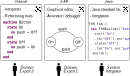
\includegraphics[width=\columnwidth]{figures/motivating-fsm}
	\caption{Shapes of an FSM language}
	\label{fig:motivating-fsm}
\end{figure}

\section{Incremental Synchronization of Metamorphic DSLs}
\td{\emph{Our} simple impl., \emph{our} patch formalism, \emph{our} dispatch, \etc}
The cornerstone artifact defining a DSL in any TS is its abstract syntax.
The way abstract syntax is expressed differs drastically from one LWB to another: Xtext\footnote{\url{https://www.eclipse.org/Xtext/}} and GEMOC~\cite{bousse2016execution} use Ecore metamodels~\cite{steinberg2008emf}; Spoofax~\cite{kats2010spoofax} uses SDF grammars~\cite{heering1989syntax}; MPS\footnote{\url{https://www.jetbrains.com/mps/}} uses \emph{concepts}; Rascal~\cite{klint2010easy} uses Algebraic Data Types (ADT); \etc.
Language embedding techniques, on the other hand, use the constructs of an host language to materialize the abstractions of a DSL in the host language itself.
In all models, concrete models are then built as instances of the corresponding abstract syntax formalism:~Ecore models, ADT values, Java constructs, \etc.
The tools defined within a given TS (\eg~an interpreter in Rascal, an editor in EMF) manipulate models in the appropriate formalism (\eg, respectively, ADT values and Ecore models).

A naive way to bridge these TS would be to define bidirectional transformations between the AS formalisms of every pair $\langle TS, TS' \rangle$.
Doing so however would break \emph{incrementality}, \ie~it would not be possible to maintain the extra information every TS holds, such as layout in a editor or runtime data when running models.
In our approach, instead, every change occuring on one side is shipped to all the other sides.
The latter then decide which parts of the changes they want to take into account.
An outline, for instance, would probably ignore most of the changes and focus on some of them. Argh.

Bridging multiple TS thus requires to ``align'' in some ways the representation of the AS of a language in these different TS.
As an illustration, the EMF and the Rascal LWB expose fundamental differences:~object-oriented vs. functional, graphs vs. trees, mutable ASG vs. immutable ASTs, cross-references vs. symbolic names, \etc.
However, it is neither possible nor desirable to establish a common formalism upon which various TS would agree:~mapping those is out of reach.

The key underlying idea of our approach is to provide the capability, at any time, to ``project'' a given model in any of its shapes and to synchronize those shapes whenever one of them is updated.
We enable the projection of a given model as an ADT value, to be manipulated in the Rascal TS, or as an Ecore model, to be manipulated in the EMF TS.

Instead, our approach keeps the TS fully independent and builds a communication bus between them.
Both representations of the same model in various TS are kept in memory to allow online synchronization of the same models manipulated by different stakeholders in different shapes.
When a changes occurs on either side, this side is responsible for generating a \emph{patch} (aka. \de or edit script~\cite{rozen2017towards}), that stores the changes on the model that have been realized on this side.
The communication bus then ships this patch to all the other sides.
Every side interprets the patch in its own way to keep the representation synchronized.
On the EMF side, for instance, the patch is interpreted as a set of changes that impact an Ecore model, while on the Rascal side it is interpreted as a set of changes that impact a value conforming to the ADT defining the AS of the language.

It is important to note that each TS may want to preserve certain information across the patches that are specific to the TS.
A textual editor in Rascal, for instance, needs to keep some of the parsing information to maintain layout whenever patches are applied.
So it should be possible to apply the patch while maintaining the extra information specific to a given TS.

Automatically generating language implementations in different TS is beyond the scope of this paper.\footnote{Indeed, this would actually require to build some kind of BX between all AS formalisms; so, nope!} Instead, given various shapes of a language, implemented by hand, we provide the means to automatically synchronize the projections of a model.

\begin{lstlisting}[label=lst:delta-adt, caption={CRUD-like \ds structure definition in Rascal}, language=Rascal]
@doc{A patch consists of a sequence of edits}
alias Patch = tuple[Id root, Edits edits];

@doc{Edits are operations attached to object identities}
alias Edits = lrel[Id obj, Edit edit];

data Edit
  = put(str field, value val)
  | unset(str field)
  | ins(str field, int pos, value val)
  | del(str field, int pos)
  | create(str class) 
  | destroy();
\end{lstlisting}

It is important to note that ``projections'' have no relation whatsoever with projectional editing.
A projection denotes the incarnation of a model in a particular shape of a language.
In \Cref{fig:motivating-fsm}, the lower part depicts three projections of the same \texttt{Button} state machine model in three shapes of the FSM language.
We use the term ``language'' to refer to the specification of a language independently from its realization in a given TS.
A concrete implementation of a language is a ``shape''.
An instance of a shape, \ie~a particular model in a particular TS, is a ``projection'' of a ``virtual'' model.
Metamorphic synchronization refers to the ability to synchronize the projections of a given model for every shapes of a language.

\begin{figure}
	\centering
	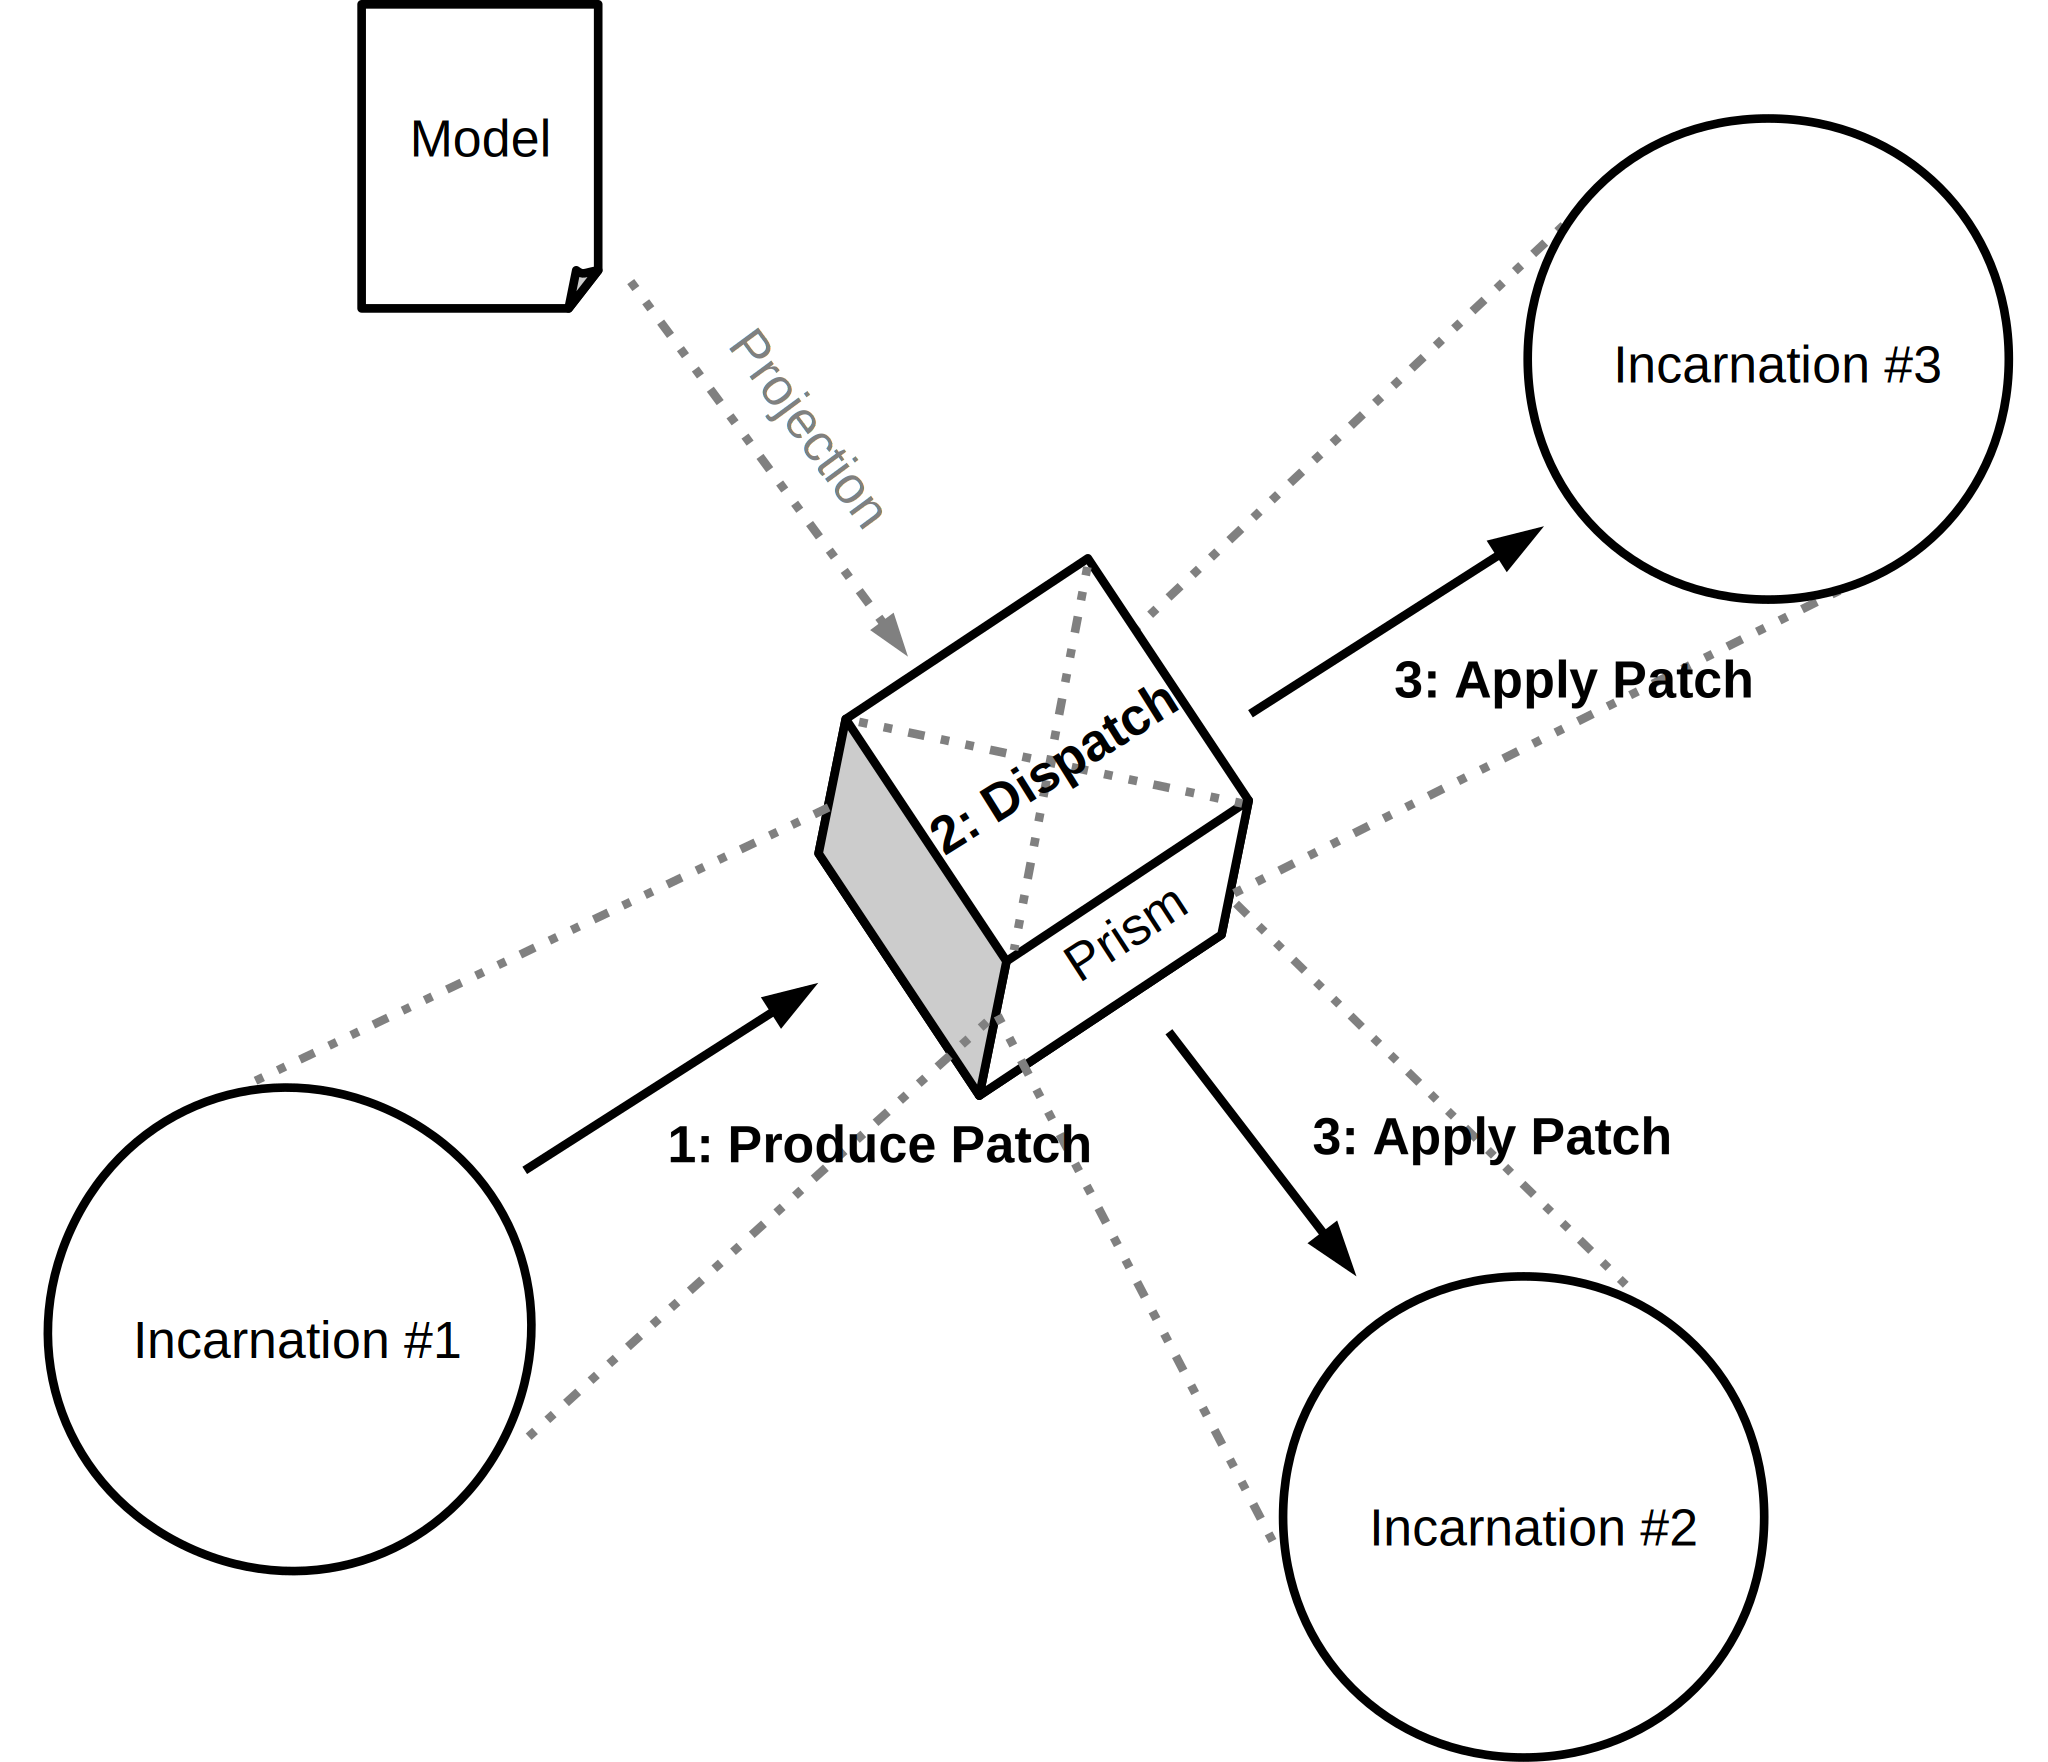
\includegraphics[width=.6\columnwidth]{figures/prism}
	\caption{\dots}
	\label{fig:prism}
\end{figure}

\section{Shapes of an FSM Language}

\begin{figure}
	\centering
	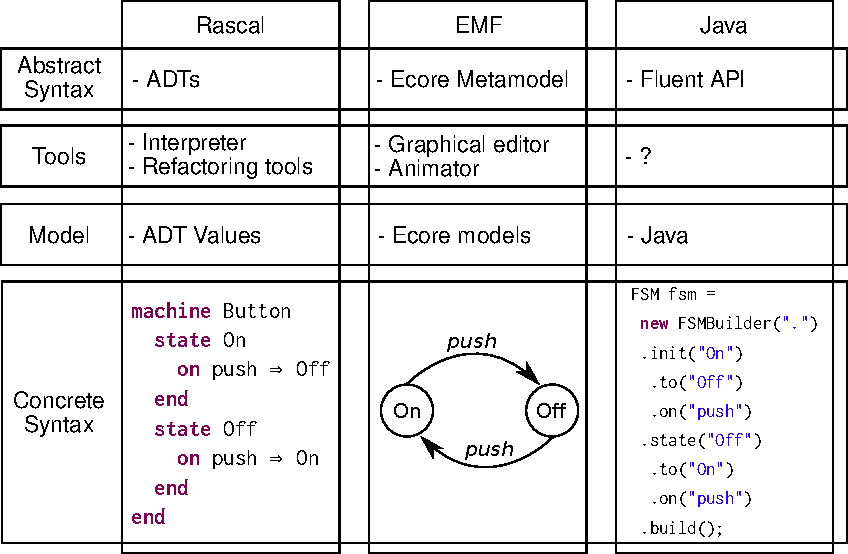
\includegraphics[width=\columnwidth]{figures/concepts-instantiated}
	\caption{\dots}
	\label{fig:concepts-instantiated}
\end{figure}

\subsection{Rascal}
\begin{minipage}{\columnwidth}
\begin{lstlisting}[label=lst:fsm-adt, caption={FSM in Rascal}, language=Rascal]
data Machine(Id uid = noId(), loc pkgURI = |http://www.example.org/myfsm|)
  = Machine(str name, list[State] states, Ref[State] initial = null());

data State(Id uid = noId())
  = State(str name, list[Trans] transitions);

data Trans(Id uid = noId())
  = Trans(str event, Ref[State] target);
\end{lstlisting}
\end{minipage}

The FSM is defined with Abstract Data Types.
Each concept of the FSM has a unique identifier.
Rascal is a tree based language and thus has no concept for references.
We defined a Abstract Data Type Ref that can be instanciated in a value containing an identifier and therefore emulate a reference.

\subsection{Ecore}
\begin{figure}
	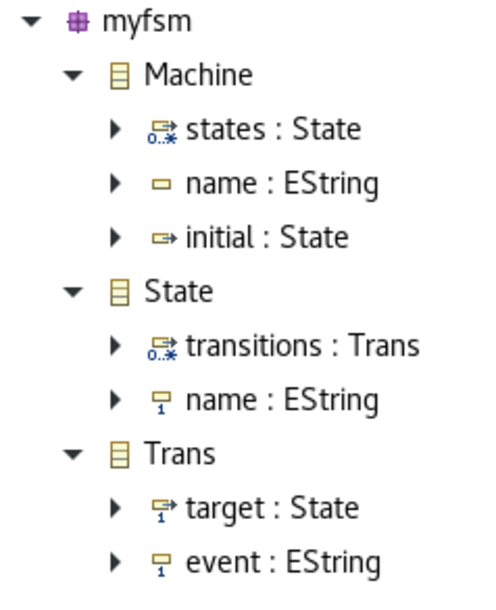
\includegraphics[width=4cm]{figures/fsm-ecore.pdf}
	\caption{Fsm in EMF---Replace with MM syntax}
	\label{fig:fsmEcore}
\end{figure}

The FSM is defined as an Ecore
Metamodel containing three EClasses representing the main con-
cepts. We define Machine as the root container EClass. It has an
EAttribute ’name’, a containment EReference ’states’ typed State
and a simple EReference ’initial’ typed State. The EClass State has
an EAttribute ’name’ and a containment EReference ’transitions’
typed Trans. The EClass Trans has an EAttibutte ’event’ and a
simple EReference ’target’ typed State.

\subsection{Java}
\begin{minipage}{\columnwidth}
\begin{lstlisting}[label=lst:fsm-api, caption={FSM in Fluent API}, language=Java]
class Fsm {
  Fsm(String name);
  State initial(String name);
  State state(String name);
  Fsm end();
}
class State {
  State state(String name);
  Transition target(String stateName);
  Fsm end();
}
class Transition {
  Transition target(String stateName);
  State on(String event);
  Fsm end();
}
\end{lstlisting}
\end{minipage}

An API is fluent if it can be used in a way that looks like a programe.
The FSM is represented as a sequence of method invocation.
The references are represented by argument of type String that allows the user to reference a State by its name.

As a fluent API is an embeded language, we need a mechanism to identified which range of a file is representing an FSM model.

A source of divergence with other Shapes of FSM is the encoding of the initial State.
We choose to represent a State by the method state() or by the method initial().
As the initial State is unique, we enforce its declaration as the first method invocation in the FSM. This solution solve the uniqueness but enforce the first state to be initial that it can be a source of divergence if models in other shape have a reference designating the initial state that is not in the first position. (if the order of State is part of the State Identifier)

\section{Discussion \& Next Steps}
\td{If we write a vision paper, there must be a vision. Next steps? Roadmap? Challenges? What should the reader gain from reading this paper?}
\td{\eg It works here for 3 ``representative'' TS. What should you have in mind if you want to do that for others? What if you want to scale for collaborative/live modeling? \etc}
\begin{itemize}
	\item Our approach goes beyond what is described here. \eg synchronizing an outline view, a debugger, live modeling, w/e; also, we are AS-centric, but one could imagine something radically different;
	\item We don’t care how the list of changes is obtained. Diff is \emph{a} way to get there (as in the Rascal implementation), but obtaining the list of changes through other means (e.g., a transaction on a tree editor in EMF) is just as valid;
	\item Our dispatch is braindead. A better dispatch may enable collaborative editing, distributed synchronization, \etc;
	\item It may or may not be possible to automatically generate a shape from another. \eg~we did it for Ecore $\leftrightarrow$ Rascal;
	\item \cite{lammel2005mappings}
\end{itemize}

\clearpage
\balance
\bibliographystyle{ACM-Reference-Format}
\bibliography{main}

\end{document}
